\documentclass[11pt]{article}
\usepackage{ifthen}
\newboolean{gitinfo}\setboolean{gitinfo}{false} % whether use gitinfo2 to provide git detail (doesn't work in Overleaf; you may also need to run RUNME.sh the first time)
 
\usepackage[truedimen, top=2cm,bottom=2cm,left=2cm,right=2cm]{geometry}
\geometry{a4paper} 
%\usepackage[parfill]{parskip}    % Activate to begin paragraphs with an empty line rather than an indent
\usepackage{graphicx}
\usepackage{amssymb}
%\usepackage{epstopdf}
%\DeclareGraphicsRule{.tif}{png}{.png}{`convert #1 `dirname #1`/`basename #1 .tif`.png}

\usepackage[table,dvipsnames]{xcolor}    % loads also �colortbl�
\definecolor{lightblue}{rgb}{0.93,0.95,1.0}
%\rowcolors{2}{blue!4}{white}
\rowcolors{1}{lightblue}{white}
\definecolor{link}{rgb}{0,0,1}
\usepackage[colorlinks,
linkcolor={link},citecolor={link},urlcolor={link},
 breaklinks, bookmarks, bookmarksopen, bookmarksnumbered
]{hyperref}
\usepackage{url}\urlstyle{sf} % rm, sf, tt or same
%% Define a new style for the urls that will use a smaller font.
\makeatletter
\def\url@smallurlstyle{%
  \@ifundefined{selectfont}{\def\UrlFont{\sf}}{\def\UrlFont{\footnotesize\sffamily}}}
\makeatother
%% Now actually use the newly defined style.
\urlstyle{smallurl}
\usepackage{PTSansNarrow} % narrow sans serif font for urls
\usepackage[scaled=.9]{inconsolata} % for texttt
\usepackage{mathpazo}
\usepackage{datetime2}\DTMsetdatestyle{iso}
\ifthenelse{\boolean{gitinfo}}{\usepackage[grumpy]{gitinfo2}}{}
\usepackage{natbib}
\usepackage{ltablex}\keepXColumns
\usepackage{sistyle}
\usepackage{array}
\usepackage[strings]{underscore} % allows hyphenation at underscores
\usepackage[nooneline,small,hypcap=true]{caption} % correct hypcap needs v 3.1 or higher
\renewcommand{\captionlabelfont}{\bfseries}
\setlength{\captionmargin}{0.5cm} \setlength{\abovecaptionskip}{3pt}

\newcommand{\note}[1]{#1} % show all notes
%\newcommand{\note}[1]{\quad} % hide all notes
\newcommand{\TODO}[1]{\note{\textcolor{blue}{\textsf{\textbf{TODO: #1}}}}}
\newcommand{\FIXME}[1]{\note{\textcolor{red}{\textsf{\textbf{FIXME: #1}}}}}
\newcommand{\CONTRIBUTORS}[1]{\note{\textcolor{BurntOrange}{\textsf{\textsl{CONTRIBUTORS: #1}}}}}
\newcommand{\ISSUE}[1]{\note{\colorbox{yellow}{\textsf{\textbf{\href{https://github.com/OceansAus/ACCESS-OM2-1-025-010deg-report/issues/#1}{ISSUE #1}}}}}}
\newcommand{\CISSUE}[1]{\note{\colorbox{gray}{\textsf{\textbf{\href{https://github.com/OceansAus/ACCESS-OM2-1-025-010deg-report/issues/#1}{ISSUE #1}}}}}}
\setlength{\fboxsep}{0pt} 
\newcommand{\param}[1]{\textsf{#1}}
\newcommand{\momlink}[2]{\href{https://github.com/mom-ocean/MOM5/search?q=#2}{#1}}
\newcommand{\momparam}[1]{\param{\momlink{#1}{#1}}}

\newcommand{\nmldiffer}[1]{#1} % no special display of differing variables
%\newcommand{\nmldiffer}[1]{\textbf{#1}} % bold display of differing variables
%\definecolor{hilite}{cmyk}{0, 0, 0.9, 0}\newcommand{\nmldiffer}[1]{\colorbox{hilite}{#1}}\setlength{\fboxsep}{0pt} % colour highlight of differing variables (requires color package)
\newcommand{\nmllink}[2]{#1} % don't link variables
% \newcommand{\nmllink}[2]{\href{https://github.com/mom-ocean/MOM5/search?q=#2}{#1}} % link variables to documentation (requires hyperref package)
\definecolor{ignore}{gray}{0.7}\newcommand{\ignored}[1]{\textcolor{ignore}{#1}} % gray display of ignored variables (requires color package)
%\newcommand{\nml}[1]{{\small\textsf{\input{local/#1}}}}
\newcommand{\nml}[1]{{\footnotesize\textsf{\input{#1}}}}
\newlength{\nmllen}\setlength{\nmllen}{8ex}
%\newcommand{\doscript}[1]{\texttt{#1}\\{\footnotesize\textsf{\input{|"#1"}}}}
\newcommand{\doscript}[1]{{\footnotesize\textsf{\input{|"#1"}}}}
%\newcommand{\doscript}[1]{{\footnotesize\textsf{\input{|"#1 > tmp.tex"}\input{tmp.tex}}}}
\newcommand{\runchanges}[1]{\subsection{#1}%
%\renewcommand{\nmllink}[2]{\href{https://github.com/mom-ocean/MOM5/search?q=#2}{#1}} % link to documentation (requires hyperref package)
\doscript{/Users/andy/anaconda/bin/python3 /Users/andy/bin/nmltab.py --format latex -dp raijin-rsync/g/data3/hh5/tmp/cosima/#1/*/ocean/input.nml}%
%%\renewcommand{\nmllink}[2]{\href{https://github.com/OceansAus/cice5/search?q=#2}{#1}} % link to documentation (requires hyperref package)
%\doscript{/Users/andy/anaconda/bin/python3 /Users/andy/bin/nmltab.py --format latex -dp raijin/g/data3/hh5/tmp/cosima/#1/*/ice/cice_in.nml}%
%\doscript{/Users/andy/anaconda/bin/python3 /Users/andy/bin/nmltab.py --format latex -dp raijin/g/data3/hh5/tmp/cosima/#1/*/ice/input_ice.nml}%
%\doscript{/Users/andy/anaconda/bin/python3 /Users/andy/bin/nmltab.py --format latex -dp raijin/g/data3/hh5/tmp/cosima/#1/*/ice/input_ice_monin.nml}%
%\doscript{/Users/andy/anaconda/bin/python3 /Users/andy/bin/nmltab.py --format latex -dp raijin/g/data3/hh5/tmp/cosima/#1/*/ice/input_ice_gfdl.nml}%
%%\renewcommand{\nmllink}[2]{\href{https://github.com/OceansAus/matm/search?q=#2}{#1}} % link to documentation (requires hyperref package)
%\doscript{/Users/andy/anaconda/bin/python3 /Users/andy/bin/nmltab.py --format latex -dp raijin/g/data3/hh5/tmp/cosima/#1/*/atmosphere/input_atm.nml}%
}

\title{ACCESS-OM2: The Consortium of Ocean-Sea Ice Modelling in Australia's global ocean and sea ice model}
\author{
Andrew Kiss, Andy Hogg, Kial Stewart, Adele Morrison, Aidan Heerdegen (ANU);\\
Nicholas Hannah (Double Precision); 
Paul Spence, Matthew England, Ryan Holmes (UNSW); \\
Russell Fiedler, Simon Marsland, Peter Oke, Siobhan O'Farrell, Christopher Chapman (CSIRO); \\
Maxim Nikurashin, Fabio Dias (UTas); 
Petra Heil (AAD \& ACE CRC, UTas); \\
Gary Brassington, Helen Beggs, Justin Freeman (BoM);
Fanghua Wu (Beijing Climate Center); \\
Stephen Griffies (GFDL); 
James Munroe (Memorial U.\ Newfoundland)\\
%Andrew Roberts (Naval Postgraduate School)\\ % or (LANL)\\
\TODO{consolidate author list and add anyone who's missing (order is arbitrary at this stage)}}
\date{\textsf{The latest version of this document is available from\\
GitHub: \url{https://github.com/OceansAus/ACCESS-OM2-1-025-010deg-report}\\
%and Overleaf: \url{https://www.overleaf.com/11449164wmwcrxynvgpx} (to use Overleaf with git, see \url{https://www.overleaf.com/blog/195-new-collaborate-online-and-offline-with-overleaf-and-git-beta}; note that this feature may be shut down in the 4th quarter of 2018: \url{https://www.overleaf.com/help/343}).\\[1ex]
%Do we want to use a private GitHub repo? see \url{https://help.github.com/articles/applying-for-an-academic-research-discount/}\\[1ex] % https://github.com/OceansAus/ACCESS-OM2-1-025-010deg-report/issues/4
\hfill{\footnotesize This version: typeset \today\ \DTMcurrenttime\ \DTMcurrentzone \\ 
\ifthenelse{\boolean{gitinfo}}{%
\hfill Last commit%
\ifthenelse{\equal{\gitDirty}{}}{:}{ (\emph{didn't commit all tracked changes}):}
git hash: \gitAbbrevHash\ 
\gitCommitterIsoDate, \\\hfill committed to branch ``\gitBranch '' by \gitCommitterName\\
\ifthenelse{\equal{\gitRoff}{}}{}{\hfill \gitRoff\ commit(s) since release \gitRel \\} 
%\gitDirty\ 
%committed by \gitCommitterName , \gitCommitterIsoDate\ \\
\hfill\textbf{NB: git hash does not reflect any uncommitted changes to this document.}\\
\hfill\textbf{\textcolor{red}{Set `gitinfo' boolean to `false' in preamble before pushing to  Overleaf.}}
}
{\hfill Set `gitinfo' boolean to `true' in preamble to show git version information (doesn't work in Overleaf; you may also need to run RUNME.sh).
}
%\TODO{automatically warn if there are uncommitted changes - eg by \url{https://www.ctan.org/pkg/latexgit}}
%\FIXME{is there any way include the pdf in the git repo and also have it show an up-to-date git hash?? --- see p12 of gitinfo2 documentation}
}}\\
\raggedright{\vspace{10ex}
\textbf{CONTRIBUTORS PLEASE NOTE:}\\
{\small
\begin{itemize}
\item please sign up with GitHub and click ``watch'' on \url{https://github.com/OceansAus/ACCESS-OM2-1-025-010deg-report} to be kept informed of discussions
\item to discuss aspects of the paper, please post an issue at \url{https://github.com/OceansAus/ACCESS-OM2-1-025-010deg-report/issues} instead of using email. 
You can tag relevant parts of the .tex file with $\backslash$ISSUE\{num\} (where ``num'' is the issue number) to link to the issue page
(change tag to $\backslash$CISSUE\{num\} if the issue is closed, so it is easily changed back if the issue is reopened).
\item note contributors for sections in the .tex file with $\backslash$CONTRIBUTORS\{\ldots\}
\item add ``to do'' items to the .tex file with $\backslash$TODO\{\ldots\}
\item note errors and problems with $\backslash$FIXME\{\ldots\} in the .tex file 
\item to make git diffs easier, please try to write each sentence in the .tex file on a separate line
\item PDF is preferred for figures (especially line plots), otherwise PNG but not JPG.
We would like all figures to be generated by a Jupyter notebook in the ``notebooks`` directory to facilitate editing and updating.
Each notebook should be in a separate subdirectory, and all its output figures should be saved in that subdirectory so we can easily tell which script generated each plot.
%Copy the ``common plot-saving code`` section from ``Template.ipynb`` to use in your notebooks. 
For latex compatibility, don't use spaces in your Jupyter notebook filename, directory name, or output image filenames. 
You'll also need to download the COSIMA Cookbook from \url{https://github.com/OceansAus/cosima-cookbook}.
Notebooks are viewable at \url{http://nbviewer.jupyter.org/github/OceansAus/ACCESS-OM2-1-025-010deg-report/tree/master/figures/}.
%See \url{https://github.com/aekiss/cosima-cookbook} for how to get git diff to work nicely with Jupyter notebooks. 
\item use a bare number (no leading v) if you do git tags (for compatibility with the gitinfo2 package used here)
\end{itemize}
}}}

\begin{document}
\maketitle
\newpage
\tableofcontents
\listoffigures

\newpage

\section{Purpose of this document}
This document serves two purposes:
\begin{enumerate}
\item This is a technical report to document the configuration and performance of the ACCESS-OM2 suite of models at 1, 0.25 and 0.1$^\circ$ horizontal resolution (\url{http://cosima.org.au/index.php/models/}), intended to be a resource for the user community (e.g. COSIMA) and readily updated. This approach was partly inspired by \citet{Griffies2015a}.
\item This will form the basis of one or more journal papers to announce and assess the performance of these models, most likely to be submitted to GMD \url{https://www.geoscientific-model-development.net}
%\TODO{decide on a suitable journal.}
%\begin{itemize}
%\item JAMES? \url{http://agupubs.onlinelibrary.wiley.com/hub/journal/10.1002/(ISSN)1942-2466/} - probably not
%\item Ocean Modelling? - probably not
%\end{itemize}
\end{enumerate}

\TODO{Auto-update figures by programatically running COSIMA notebooks}, so you could have a jenkins job or somesuch checking the COSIMA tech paper notebooks are all up to date and working correctly
\url{http://tritemio.github.io/smbits/2016/01/02/execute-notebooks/}

\TODO{copy things from ARCCSS workshop poster, AMOS2018 talk, Bluelink talk, COSIMA workshop}

\section{Introduction}
This technical report documents the ACCESS-OM2 ocean-sea ice model at nominal horizontal resolutions of $1^\circ$, $0.25^\circ$ and $0.1^\circ$.

\section{Model Configuration}
\CONTRIBUTORS{Andrew Kiss to coordinate}

\subsection{Overview}

MOM, CICE, OASIS, JRA55

\url{http://www.mom-ocean.science} \TODO{move to new web location}

\subsection{MOM configuration}
MOM parameters for the three model resolutions are tabulated in Appendix~\ref{S:mom-namelist}.
We discuss the choices of key parameters here.


\TODO{cannibalise NCMAS application}

%Note hazards of tuning? \citet{DommengetRezny2018a}

%see /Users/andy/Documents/COSIMA/github/aekiss/namelist-check/namelist-meeting-2018-04-06/Fabio2018_Namelist_meeting.pdf

\subsubsection{Vertical grid}

\begin{table}
\newcolumntype{R}{>{\raggedleft\arraybackslash}p{13ex}}
\begin{tabularx}{\linewidth}{XRRRR}
\hline
Model	 & 	$n$	&	$\Delta z_\text{min}$ (m)	& 	$\Delta z_\text{max}$ (m)	& 	$H_\text{max}$ (m)	\\
\hline\endfirsthead
\hline
Model	 & 	$n$	&	$\Delta z_\text{min}$ (m)	& 	$\Delta z_\text{max}$ (m)	& 	$H_\text{max}$ (m)	\\
\hline\endhead
ACCESS-OM2		&	50	&	10.0	&	334.7	&	6000.0\\	% ncdump /short/v45/aek156/access-om2/input/mom_1deg/ocean_vgrid.nc
ACCESS-OM2-025	&	50	&	10.1	&	209.9	&	5500.0\\	% ncdump /short/v45/aek156/access-om2/input/mom_025deg/ocean_vgrid.nc
ACCESS-OM2-01	&	75	&	1.1	&	198.4	&	5808.7\\	% ncdump /short/v45/aek156/access-om2/input/mom_01deg/ocean_vgrid.nc
\hline
\end{tabularx}
\caption{Vertical grid parameters: $n$ levels, with spacing of $\Delta z_\text{min}$ and $\Delta z_\text{max}$ at the surface and maximum depth $H_\text{max}$, respectively.\TODO{these are discretised values from ocean_vgrid.nc - check that I'm correctly using the notation in \citet{StewartHoggGriffiesHeerdegenWardSpenceEngland2017a}}}\label{T:vgrid}
\end{table}
See table~\ref{T:vgrid}.

Discuss KDS vertical grid \citet{StewartHoggGriffiesHeerdegenWardSpenceEngland2017a}

\TODO{update? Kial is setting up KDS50 at 1$^\circ$}

discuss partial cells

% NB: z levels are the odd entries in ocean_vgrid.nc (counting from zero)
% ocean_grids.F90 line 297: size of dimension zeta in ocean_vgrid.nc is 2*nk+1
% ocean_grids.F90 line 446,661: T points (zt) at zeta(2k-1), w points (zw) at zeta(2k), k=1,nk  [NB in line 661,2 Grid%zt,Grid%zw ignore initial 0 in data]

% [ ( <paste ncdump> ) (,) () replace pop cvx exec ] 0:2: pick dup diff

%1deg 0:2: pick dup diff
%2: rwL 51 array   [ 0 10 20 30 40 50 60 70 80 90 100 110 120 130 140 150 160 170 180 190 200 210.92337 229.097885 261.06488 312.015594 385.283 482.015594 601.06488 739.0979 890.923401 1050 1210.26978 1372.68738 1539.3479 1712.24194 1893.20642 2083.87964 2285.66113 2499.67627 2726.74976 2967.38452 3221.74976 3489.67627 3770.66113 4063.87964 4368.20654 4682.2417 5004.34814 5332.6875 5665.26953 6000 ]
%1: rwL 50 array   [ 10 10 10 10 10 10 10 10 10 10 10 10 10 10 10 10 10 10 10 10 10.9233704 18.1745148 31.9669952 50.9507141 73.267395 96.732605 119.049286 138.03302 151.8255 159.076599 160.269775 162.417603 166.660522 172.894043 180.964478 190.673218 201.781494 214.015137 227.073486 240.634766 254.365234 267.926514 280.984863 293.218506 304.326904 314.035156 322.106445 328.339355 332.582031 334.730469 ]

%025deg 0:2: pick dup diff
%2: rwL 51 array   [ 0 10.0671 20.16 30.2889 40.4674 50.7148 61.0575 71.5323 82.1899 93.1001 104.359703 116.101402 128.507599 141.827606 156.400208 172.683105 191.287704 213.020096 238.922699 270.309509 308.779297 356.186401 414.545685 485.854401 571.842773 673.697571 791.842773 925.85437 1074.54565 1236.1864 1408.7793 1590.30957 1778.92273 1973.02014 2171.2876 2372.68311 2576.40015 2781.82764 2988.50757 3196.10156 3404.35962 3613.1 3822.19 4031.53223 4241.05762 4450.71484 4660.46729 4870.28906 5080.16 5290.06689 5500 ]
%1: rwL 50 array   [ 10.0671 10.0929 10.1289005 10.1784992 10.2474022 10.3426971 10.4748039 10.6576 10.9101944 11.2596054 11.7416992 12.4061966 13.3200073 14.5726013 16.2828979 18.604599 21.7323914 25.9026031 31.3868103 38.4697876 47.4071045 58.3592834 71.3087158 85.9883728 101.854797 118.145203 134.011597 148.691284 161.640747 172.592896 181.530273 188.613159 194.097412 198.267456 201.395508 203.717041 205.42749 206.679932 207.594 208.258057 208.740479 209.089844 209.342285 209.525391 209.657227 209.752441 209.821777 209.871094 209.906738 209.933105 ]

%01deg 0:2: pick dup diff
%2: rwL 76 array   [ 0 1.08256149 2.27890778 3.60099745 5.06204557 6.67665529 8.4609642 10.4328051 12.6118832 15.0199728 17.6811333 20.6219482 23.8717937 27.4631233 31.4317913 35.8174057 40.6637268 46.0190773 51.9368439 58.4759598 65.7015076 73.6853256 82.5067 92.2530746 103.02092 114.916573 128.057159 142.571671 158.60199 176.304016 195.848892 217.424164 241.234985 267.50528 296.478699 328.419617 363.613617 402.367523 445.009155 491.885895 543.362488 599.817383 661.637634 729.212 802.921631 883.129395 970.167 1064.32043 1165.81555 1274.80347 1391.34875 1515.42017 1646.88733 1785.52197 1931.0061 2082.94434 2240.88135 2404.32104 2572.74536 2745.63306 2922.4751 3102.7876 3286.11914 3472.05786 3660.23291 3850.31543 4042.0166 4235.08643 4429.30811 4624.49707 4820.49658 5017.17334 5214.41455 5412.12598 5610.229 5808.65674 ]
%1: rwL 75 array   [ 1.08256149 1.19634628 1.32208967 1.46104813 1.61460972 1.78430891 1.97184086 2.1790781 2.40808964 2.66116047 2.94081497 3.2498455 3.59132957 3.96866798 4.3856144 4.84632111 5.35535049 5.91776657 6.53911591 7.22554779 7.98381805 8.82137299 9.74637604 10.7678452 11.8956528 13.1405869 14.5145111 16.0303192 17.7020264 19.5448761 21.5752716 23.8108215 26.2702942 28.9734192 31.940918 35.194 38.7539063 42.6416321 46.8767395 51.476593 56.454895 61.8202515 67.5743408 73.7096558 80.2077637 87.0376 94.1534424 101.495117 108.987915 116.545288 124.071411 131.467163 138.634644 145.484131 151.938232 157.937012 163.439697 168.424316 172.887695 176.842041 180.3125 183.331543 185.938721 188.175049 190.08252 191.701172 193.069824 194.22168 195.188965 195.999512 196.676758 197.241211 197.711426 198.103027 198.427734 ]

ACCESS-OM2 uses GFDL50 \FIXME{wrong? doesn't match GFDL50 in table 1 of \citet{StewartHoggGriffiesHeerdegenWardSpenceEngland2017a}} 50 levels, 10.0m spacing in top 200m then increasing smoothly to 334.7m by the bottom at 6000m. % ncdump /short/v45/aek156/access-om2/input/mom_1deg/ocean_vgrid.nc

ACCESS-OM2-025 uses KDS50 \FIXME{wrong? doesn't match KDS50 in table 1 of \citet{StewartHoggGriffiesHeerdegenWardSpenceEngland2017a}} 50 levels, 10.1m spacing at surface, increasing smoothly to 209.9m by the bottom at 5500m. % ncdump /short/v45/aek156/access-om2/input/mom_025deg/ocean_vgrid.nc

ACCESS-OM2-01: KDS75 \TODO{check: maximum spacing and depth slightly different from KDS75} 75 levels, 1.1m spacing at surface, increasing smoothly to 198.4m by the bottom at 5808.7m. % ncdump /short/v45/aek156/access-om2/input/mom_01deg/ocean_vgrid.nc


\TODO{figure showing grid spacing vs depth for ACCESS_OM2 models and others for comparison} 

\subsubsection{Horizontal grid}
% ncdump -h /short/v45/aek156/access-om2/input/mom_1deg/ocean_hgrid.nc
% ncdump -h /short/v45/aek156/access-om2/input/mom_025deg/ocean_hgrid.nc
% ncdump -h /short/v45/aek156/access-om2/input/mom_01deg/ocean_hgrid.nc

The grid covers the global ocean, extending from the north pole to 81$^\circ$S.
The grid is Mercator between 65$^\circ$N -- 65$^\circ$S, and tripolar \citep{Murray1996a} north of 65$^\circ$N, with tripoles placed on land at 65$^\circ$N and -100$^\circ$E, 80$^\circ$E. % see windrotation.ipynb
\TODO{describe spacing south of 65S}

\TODO{explain grid refinement at equator --- 1$^\circ$ only?}

\TODO{plots of x and y grid spacing in the three models}

\url{https://github.com/mom-ocean/MOM5/blob/master/doc/web/user_guide.md}: ``The grid_spec file [/short/v45/aek156/access-om2/control/01deg_jra55_ryf] contains the following horizontal grid information: geographic location of T, E, C and N-cell (Tracer, East, Corner, and North cells), half and full cell lengths (in meters), rotation information between logical (i.e., grid oriented) and geographic east of cell. The complete description of the horizontal grid and namelist option is available in hgrid''

\subsubsection{Bathymetry}
\CONTRIBUTORS{Russ Fiedler}

There are no ice cavities as these are not supported in MOM5.1. Topography ends at a vertical wall at the ice shelf edge (the calving line, not the grounding line).

\paragraph{1$^\circ$ and 0.25$^\circ$}

\paragraph{0.1$^\circ$}

based on Gebco2014 30sec gridded data % original data located at /g/data3/hh5/tmp/cosima/bathymetry/gebco.nc
\FIXME{which version?} \url{http://www.gebco.net/data_and_products/gridded_bathymetry_data/gebco_30_second_grid/}
The topo data used in the runs is /short/v45/aek156/access-om2/input/mom_01deg/topog.nc

\TODO{check if this relevant to the bathy file we use:}
 "Enforced minimum of 7 levels (approx 10m). Excavated not filled in so land mask kept. Partial cells: Enforced thickness of max(10,0.2*dz). If partial cell were thinner than half this then the cell was removed." ( /g/data3/hh5/tmp/cosima/bathymetry/README )

Minimum depth = 10m

Partial cells:
ncdump -h /short/v45/aek156/access-om2/input/mom_01deg/topog.nc
yields 
		depth:minimum_depth = 10.43281f ;
		depth:minimum_levels = 7 ;
		depth:min_thick = 10.f ;
		depth:min_frac = 0.2f ;

\subsubsection{Other model settings}
SGS parameterisations, mixed layer, bottom boundary layer, etc

horizontal and vertical friction, lateral boundary conditions

equation of state

\subsection{CICE sea ice model configuration}
CICE parameters for the three model resolutions are tabulated in Appendix~\ref{S:cice-namelist}.
We discuss the choices of key parameters here.

CICE parameter sensitivities: \citet{UrregoBlancoUrbanHunkeTurnerJeffery2016a}

cf. Andrew Roberts RASM cice namelist (Petra email 6 June) \TODO{get permisssion}
which was used in \citet{CassanoDuVivierRobertsHughesSeefeldtBrunkeCraigFiselGutowski2017a,HammanNijssenRobertsCraigMaslowskiOsinski2017a,JinDealMaslowskiMatraiRobertsOsinskiLeeFrantsElliott2018a,Roberts2018a}
see Appendix~\ref{S:rasm-namelist}

See Andrew Roberts' comments on \citet{RobertsCraigMaslowskiOsinskiDuvivierHughesNijssenCassanoBrunke2015a} in email from Petra email 6 June --- inertial coupling can be essential for stability

\subsubsection{Thickness redistribution}

4 ice layers + 1 snow

5 thickness categories. 
We use \param{kcatbound=0}, so lower bound of ice categories is 0, 0.64, 1.39, 2.47, 4.57m \citep[][table 2]{HunkeLipscombTurnerJefferyElliott2015a-CICE5p1}.
For ridging we use we use \param{krdg_partic=1}.

\subsubsection{Dynamics}
\TODO{check I (AK) haven't misunderstood anything here --- this is based on only a quick skim of most of these papers}

We are currently using ``classic EVP'' (\param{kdyn = 1}, \param{revised_evp = .false.}) \citep{HunkeDukowicz1997a,HunkeDukowicz2002a,Hunke2001a}.
This represents the ice by a viscoplastic (VP) rheology, to which a fictitious elastic term is added to facilitate efficient numerical convergence to the viscoplastic solution via damped elastic waves which are supposed to decay to negligible amplitude during \param{ndte} sub-timesteps within each dynamic timestep \citep[][sections~3.5.2 and~4.4]{HunkeLipscombTurnerJefferyElliott2015a-CICE5p1}.
Another CICE option is the ``revised EVP'' method \citep[section~3.5.3]{BouillonFichefetLegatMadec2013a, HunkeLipscombTurnerJefferyElliott2015a-CICE5p1} which corrects an error in the ``classic EVP'' stress formulation and may also improve the convergence rate of the elastic sub-timesteps and reduce the incidence of spurious grid-aligned linear kinematic features (``leads'').
\TODO{try this out?}
\citet{BouillonFichefetLegatMadec2013a} argue that this is superior to using ``classic EVP'', but see warnings by \citet{KimmritzLoschDanilov2017a, KimmritzDanilovLosch2015a} that numerical instability may dominate over convergence as the greatest source of error.\FIXME{wrong references? they don't say this as far as I can see.}

There is an ongoing debate regarding the suitability of viscoplastic ice rheology, particularly to represent on fine scales \citep{Nye1973a, WeissSchulsonStern2007a, LindsayZhangRothrock2003a,KwokHunkeMaslowskiMenemenlisZhang2008a, GirardWeissMolinesBarnierBouillon2009a, DansereauWeissSaramitoLattes2016a, HutterLoschMenemenlis2018a}. 
An alternative supported by CICE is the elastic-anisotropic-plastic (EAP) model \citep{WeissSchulson2009a, WilchinskyFeltham2006a, TsamadosFelthamWilchinsky2013a}, but this seems relatively untested and uncalibrated at this stage.

If we accept the VP formulation, there is also the question of how well the EVP sub-timesteping converges to the VP solution with no residual elastic wave effects.
Like many comparable models we use \param{ndte=120} sub-timestep iterations, but \citet{LoschDanilov2012a, LemieuxKnollTremblayHollandLosch2012a, KimmritzLoschDanilov2017a, KimmritzDanilovLosch2015a} show that full convergence may take thousands of iterations even with the revised EVP method (particularly at high resolution), which would be prohibitively expensive. We must therefore expect our sea ice stress distribution to contain artefacts due to residual elastic waves. These artefacts may include spurious grid-scale noise and long linear features in the shear and divergence fields \citep{LemieuxKnollTremblayHollandLosch2012a}.

see \citet{LemieuxTremblay2009a}

discuss linear kinematic features (leads): \citet{HutchingsHeilHibler2005a, WangDanilovJungKaleschkeWernecke2016a, WangWang2009a, LoschFuchsLemieuxVanselow2014a}

turning angle is set to zero --- is this reasonable? see \citet{ParkStewart2016a, McPhee2008a, Lepparanta2011a} --- we are using 10m ageostrophic winds and can resolve the ocean Ekman layer.

Ice-ocean drag coefficient: we use \param{dragio=0.00536}, very close to the measured value of 0.0054 measured at 0.5\,m below first-year landfast ice by \citet{ShirasawaIngram1997a}.
A wide range of values have been used in the literature \citep[][table~5.3]{LuLiChengLepparanta2011a, MartinsonWamser1990a, Lepparanta2011a}, but the coefficient also depends on the water velocity and depth at which it is measured, the ice roughness, and the upper ocean stratification \citep{Lepparanta2011a, WatersBruno1995a}.

\subsubsection{Thermodynamics}
mushy ice: \citet{TurnerHunkeBitz2013a}

See Andrew Roberts' comments on mushy thermo in email from Petra email 6 June

melt ponds?
See Andrew Roberts' comments on melt ponds in email from Petra email 6 June

\subsection{OASIS}

OASIS3-MCT or OASIS-MCT2?

Nic's work on ESMF regridding

Regridding method - \url{https://github.com/OceansAus/access-om2/wiki/Creating-Remapping-Weights}

Should we use high-frequency coupling? CICE flag \param{highfreq} implements the RASM coupling method of \citet{RobertsCraigMaslowskiOsinskiDuvivierHughesNijssenCassanoBrunke2015a}; also see \url{http://www.oc.nps.edu/NAME/RASM_overview.pdf}

\subsection{Forcing}
JRA55-do v1.3 atmospheric forcing (1984-5, 1990-1 or 2003-4 repeat-year, 0.5625$^\circ$, 3-hourly) in addition to CORE NYF (2$^\circ$, 6-hourly)

\subsubsection{JRA55-do and repeat-year forcing}

JRA55-do user manual: \citet{TsujinoUrakawaNakanoSmallKimYeagerDanabasogluSuzukiBamber2018a}

Data available from \url{https://esgf-node.llnl.gov/search/input4mips/?institution_id=MRI}
and on NCI at /g/data1/ua8/JRA55-do/RYF/v1-3/*.nc

For the latest information on the dataset status and citation: \url{http://goo.gl/r8up31}.

see \url{http://amaterasu.ees.hokudai.ac.jp/~tsujino/JRA55-do-v1.3/00README_v1_3.1st}
JRA-55: \citet{KobayashiOtaHaradaEbitaMoriyaOnodaOnogiKamahoriKobayashi2015a}
JRA55-do: \citet{Tsujino2015a, Tsujino2015b, Tsujino2016a, TsujinoETAL2018a}, \citet{TsujinoUrakawaSuzukiKomuroSmallKimYeagerDanabasogluGriffies2016a}

\url{http://www.clivar.org/omdp/japan2016}

JRA55-do version 1.3 provides
3-hourly liquid and solid precipitation, downwelling surface longwave and shortwave radiation, sea level pressure, 10m wind velocity, specific humidity and air temperature 
on a TL319 grid, 0.5625$^\circ$ (9/16$^\circ$) resolution,
and daily river flux at 0.25$^\circ$ resolution.

\TODO{check: what do we use for glacier runoff? groundwater? evaporation? upwelling longwave radiation?}

``Runoff from Greenland and Antarctica are replaced by climatological runoff.
Greenland runoff is based on \citet{BamberBroekeEttemaLenaertsRignot2012a} and Antarctica runoff
is based on \citet{DepoorterBamberGriggsLenaertsLigtenbergBroekeMoholdt2013a}.'' (\url{http://amaterasu.ees.hokudai.ac.jp/~tsujino/JRA55-do-v1.3/00README_v1_3.1st})

we made a start on this: \url{https://github.com/OceansAus/matm/issues/5}

should we / do we use this for runoff? \citet{SuzukiYamazakiTsujinoKomuroNakanoUrakawa2017a}

currently fresh water is input at the ice shelf edges.

cf.\ runoff (iceberg discharge scheme) used in ACCESS-CM2 - see AMOS2018 notes on Dave Bi's talk and \url{https://accessdev.nci.org.au/trac/wiki/CMIP6workshop}
--- this is discharged only at the surface.

Runoff - incl distributed iceberg melt? Ask Adele? basal melt needs to be at depth - notebook p561. We have the data but waiting on it being published. 
Veronique has regridded this - see email 2017-11-16 \citet{MerinoLeSommerDurandJourdainMadecMathiotTournadre2016a} and
\citet{DepoorterBamberGriggsLenaertsLigtenbergBroekeMoholdt2013a}
Paul: ``The Antarctic ice berg data is published and the data is publicly available here: 
\url{http://neichin.github.io/personalweb/publications/}
However, the Antarctic basal melt fluxes are not published yet and the data has not been made public.''
Also see \citet{MerinoJourdainLe-SommerGoosseMathiotDurand2018a, Donat-MagninJourdainSpenceLe-SommerGalleeDurand2017a, MathiotJenkinsHarrisMadec2017a}

Runoff - what range of depths is used? Top 4 levels??


discuss choice of year for RYF --- will use 1984-5 for high-res runs -- refer to Kial's paper

These 12-month periods were identified as particularly "neutral":
1 May 1984 - 30 April 1985,
1 May 1990 - 30 April 1991,
1 May 2003 - 29 April 2004 (we keep 29 Feb 2004 and ditch 30 April 2004 so as to keep 365 days per year).
We have run ocean-sea ice spinups forced by all three JRA55-do v1.3 repeat years at 1$^\circ$ but we are concentrating on 1984-5 for the 1/10$^\circ$ spinup as it has less of the warming signal and also gives us more of the JRA55 dataset for subsequent interannual runs.

Kial's email 2018-03-05:
\begin{quote}
-1st of January is in the peak of the northern winter and southern summer, meaning the variability in forcing fields (ie. weather) is quite high. This is a problem for surface buoyancy fluxes in the north Atlantic and Labrador \& Nordic Sea regions, where NADW formation is notoriously sensitive to changes in surface forcing. The day of the year with lowest variability (least weather) is going to be closer to the equinoxes, and in JRA55 DO it turns out to be 1 May. 

-The three candidate years have been selected as the 12-month periods with climate indices closest to neutral. The climate indices of interest are the SOI, SAM and NAO. Removing the criteria that a 12-month period follows the calendar year allows us to find "years" that are closer to climatologically neutral.

-Having the jump at 1 May allows us to run the model harder. The model tends to fall over at 1 Jan if the jump is there, meaning we have to back off the timestep and nurse it through. Having the jump at 1 May does not require any such nursing. Currently we are running the ACCESS-OM2 1$^\circ$ with 5400 sec timesteps from initialization and getting through ~90 years per day.
\end{quote}

\subsubsection{CORE-NYF}

\subsubsection{Restoring}

sea surface salinity restoring: salt_sfc_restore.nc from World Ocean Atlas 2013 v2 \url{https://www.nodc.noaa.gov/OC5/woa13/}; % ncdump -h salt_sfc_restore.nc gives: This salinity distribution is based on WOA13v2 where the land values are filled in with a conjugate gradient method. It is a simple average of land-filled salinity data at the depth of 0 and 10 meters.
timescale set by salt_restore_tscale (we use 10 days) but what really matters is piston velocity

15m/300day ie 0.05m/day is GFDL's standard piston velocity (Griffies, 12 April 2018)

with 1.1m top cell and 10 days, we have 0.11 m/day ie restoring twice as strongly as GFDL

see \url{https://github.com/OceansAus/access-om2/issues/52} and \url{http://www.earthsystemmodeling.org/esmf_releases/last_built/ESMF_refdoc/node3.html#SECTION03020000000000000000}

2nd order conservative interpolation:
\citet{KritsikisAechtnerMeurdesoifDubos2017a}

\subsubsection{Bulk formulas used}

- relative or absolute wind? see \citet{WuZhaiWang2017a} and  \url{https://arccss.slack.com/archives/C6PP0GU9Y/p1511825314000106?thread_ts=1511802000.000465&cid=C6PP0GU9Y}
and \url{https://jra55-do.slack.com/archives/C7LEZT4KY/p1511963905000047}
- we are using relative wind - but where is this set?

\subsubsection{YATM / MATM}
MATM parameters for the three model resolutions are tabulated in Appendix~\ref{S:matm-namelist}.

\subsection{Initial conditions and spinup}
Initial condition is from World Ocean Atlas 2013 v2 \url{https://www.nodc.noaa.gov/OC5/woa13/}.

What's the sea ice initial condition? 3m at pole, dropping off with latitude equatorward?? - Siobhan - 
parameter ice\_ic = 'default' 
'default'  = latitude and sst dependent
\url{https://github.com/OceansAus/cice5/blob/5583ce54fd8822c1b8aef0549090167ca5f36d10/source/ice_init.F90#L23}
sets up ice where SST is cold, max 3m thick...?
\url{https://github.com/OceansAus/cice5/blob/5583ce54fd8822c1b8aef0549090167ca5f36d10/source/ice_init.F90#L1538}

\subsubsection{Online runoff remapping via kdtree}

\subsection{Model computational details and performance}

\citet{CraigMickelsonHunkeBailey2014a}?

cf. \ MOM-SIS-01: 50--60kSU/day? - check with Andy

1/10$^\circ$: 1200 PUs for CICE + 4358 PUs for MOM + 1 for MATM \TODO{update}

\TODO{cf. Matt Chamberlain's 2016 talk: global MOM-SIS at 1/10$^\circ$ and 50 levels, 960 CPUs (50x23 layout, 200 masked), dt=720s, month $\sim$100min: \url{http://cosima.org.au/wp-content/uploads/2016/06/ofam_global.mac_.pdf} --- this is as fast as ACCESS-OM2-01 but about 6x cheaper!}

\subsection{Comparison with similar models}
Namelists of MOM-based models are compared in Appendix~\ref{S:namelist-model-comparisons}.


\begin{table}%[htdp]
\caption{ACCESS-OM2 updates and extends ACCESS-OM and OFAM3}
\begin{center}
\begin{tabular}{|c|c|c|c|}
\hline
& \textbf{ACCESS-OM} & \textbf{OFAM3} & \textbf{ACCESS-OM2}\\
\hline
Ocean & MOM~4.1 & MOM~4.1 & MOM~\textbf{5.1}\\
Sea ice & CICE~4.1 & --- & CICE~\textbf{5.1}\\
%Atmosphere & MATM & --- & MATM\\
%Forcing & & JRA55-do (XX$^\circ$, 6hr)&\\\
Coupler & OASIS~3.25 & --- & OASIS \textbf{3-MCT}\\
%Interpolation & SCRIPP & --- & ESMF \\
Grid & global tripolar, $z^*$ & 75$^\circ$S--75$^\circ$N only, $z^*$ & global tripolar, $z^*$\\
Resolution & 
1$^\circ$, 360$\times$300$\times$50 & 
\parbox[][][c]{22ex}{%
0.1$^\circ$, 3600$\times$1500$\times$51, $\Delta z$=5 -- 1000m 
} &
\parbox[][][c]{22ex}{%
1$^\circ$, 360$\times$300$\times\\$(50, 75 or 100 levels)\\
or\\0.25$^\circ$,~1440$\times$1080$\times$50,\\$\Delta z=10.1$ -- 210m\\
or\\\textbf{0.1$^\circ$, 3600$\times$2700$\times$75, $\Delta z$=1.1 -- 198m\\[-1ex]}}\\
%Resolution & 1$^\circ$, 360$\times$300$\times$50 & \parbox[][][c]{20ex}{0.1$^\circ$ near Aust, up to 2$^\circ$ elsewhere, 1191$\times$968$\times$47} & \parbox[][][c]{20ex}{1$^\circ$, 360$\times$300$\times\\$(50, 75 or 100 levels)\\or\\0.25$^\circ$,~1440$\times$1080$\times$50\\or\\0.1$^\circ$, 3600$\times$2700$\times$75}\\
%Top layer thickness & ? & 5\,m 
%\rowcolor{white}& & &                                                  0.25$^\circ$, 1440$\times$1080$\times$50\\
%& & &                                                  0.1$^\circ$, 3600$\times$2700$\times$75\\
%Initial condition & WOA~2005 & global CARS & WOA~2013~v2\\
%\vspace{2ex}
\hline
\end{tabular}
\end{center}
\label{T:access-om-ofam3-access-om2}
\end{table}

\subsubsection{GFDL CM2, CM2.5, CM2.6}
cf. CM2-1deg CM2.5 CM2.6 (they were MOM v5) and discuss resolving eddies: \citet{GriffiesWintonAndersonBensonDelworthDufourDunneGoddardMorrison2015a}
\citet{DelworthRosatiAndersonAdcroftBalajiBensonDixonGriffiesLee2012a}
\citet{DunneJohnAdcroftGriffiesHallbergShevliakovaStoufferCookeDunne2012a}
\citet{Griffies2015a}

cf.\ CORE \citep{GriffiesBiastochBoningBryanDanabasogluChassignetEnglandGerdesHaak2009a}, CORE-II \citep{DanabasogluYeagerBaileyBehrensBentsenBiBiastochBoningBozec2014a}

minimum depth = 40m ?

\subsubsection{ACCESS, ACCESS-CM2, ACCESS-ESM}
See \url{https://accessdev.nci.org.au/trac/wiki/CMIP6workshop} --- Marsland will be making slides available on Subversion repo.
There's an ACCESS-CM2 report available - ask Arnold Sullivan.
And data is available on NCI to members of p66 and NCI access groups

cf. ACCESS \citet{BiDixMarslandOFarrellRashidUotilaHirstKowalczykGolebiewski2013a, BiMarslandUotilaOFarrellFiedlerSullivanGriffiesZhouHirst2013a, DixVohralikBiRashidMarslandOFarrellUotilaHirstKowalczyk2013a}

\citet{BiMarslandUotilaOFarrellFiedlerSullivanGriffiesZhouHirst2013a}

cf. ACCESS-CM2 \citet{BiYanSullivan2016a}, \url{http://cosima.org.au/wp-content/uploads/2016/06/BI-COSIMA-Hobart-20160526.ppt.pdf} - Uses same MOM, CICE and OASIS versions as ACCESS-CM2

cf. ACCESS-ESM \url{https://www.google.com.au/url?sa=t&rct=j&q=&esrc=s&source=web&cd=2&ved=0ahUKEwjvjsmH0rjZAhWEnpQKHb7VC-EQFgg0MAE&url=https%3A%2F%2Faccessdev.nci.org.au%2Ftrac%2Fraw-attachment%2Fwiki%2FScienceDay%2Fziehn_access_esm1.pdf&usg=AOvVaw1bYwLzey6vpy7g6v7W0aF0}

\subsubsection{OFAM3}
cf. OFAM3 namelists - see Matt Chamberlain's email 28 May 2018

cf. oceanMAPS3.0  \url{http://cosima.org.au/wp-content/uploads/2016/06/Brassington_Ocean_modelling_and_forecasting_v3.pptx.pdf} % /Users/andy/Documents/COSIMA/COSIMA workshop 26-27 May 2016/Gary Brassington (BoM) Brassington_Ocean_modelling_and_forecasting_v3.pptx.pdf

The vertical resolution has also been improved relative to OFAM3 \citep{OkeETAL2013a} at nearly all depths, particularly at the surface and in the deep ocean, with 75 levels ranging from 1.1m thick at the surface to 198m thick at 5808m (compared to 51 levels ranging from 5m to 1000m thick currently in OFAM3/Bluelink). Of particular relevance for coastal studies is the improved vertical resolution in the upper ocean, with 31 levels in the top 200m and a minimum water depth of 10m (rather than 24 levels and a minimum depth of 15m for OFAM3), providing better resolution of shelf processes and a closer match to coastlines.

\subsubsection{MOM-SIS-01}
cf. MOM-SIS-01 \citet{SpenceHolmesHoggGriffiesStewartEngland2017a} - forced by 2$^\circ$ CORE NYF - 75 levels; ACCESS-OM2-01 has newer bathy, CICE, JRA55-do, and probably different vertical grid

\subsubsection{UKMO GO6, GO7}
cf UKMO GO6, GO7 \citet{StorkeyBlakerMathiotMegannAksenovBlockleyCalvertGrahamHewitt2018a} - based on NEMO.

GO7 has cavities under the ice shelves, whereas GO6 is similar to ACCESS-OM2-x in having no cavities and fresh water input at the ice shelf edges.

\subsubsection{RASM?}


\section{Model evaluation}
 \CONTRIBUTORS{Andy Hogg to coordinate}

use obs dataset and methods from CLIVAR Repository for Evaluating Ocean Simulations? \url{http://www.clivar.org/clivar-panels/omdp/reos}
 
 cf Ocean Modelling CORE-II Special Issue (Virtual) \url{http://www.sciencedirect.com/science/journal/14635003/vsi/10PSR6J3BV4}

OMIP - \citet{GriffiesETAL2016a} - does BOM/CSIRO already have code to do this for CMIP6? ask Marsland

cf \citet{OkeETAL2013a}

cf \url{http://www.cesm.ucar.edu/working_groups/Ocean/metrics.html}?

cf esmvaltool \url{https://www.esmvaltool.org/}?

See Fanghua's observation comparison notebooks (should be on github) and also her presentation from 2018-01-25
and \url{https://github.com/FanghuaWu/cosima-cookbook/tree/master/notebooks}

maps of Smagorinsky biharmonic lateral viscosity? what is the viscous WBC width this implies?
- note that lateral visc is increased near western boundary, even in 0.1$^\circ$ model:  This is set by \param{ncar_boundary_scaling} in `MOM5/src/mom5/ocean_param/lateral/ocean_bihgen_friction.F90`

see HighResMIP \citep{HaarsmaETAL2016a}

\subsection{Barotropic streamfunction}
late separation of Kuroshio - cf. \citet{ColindeVerdiereOllitrault2016a}
seems to be due to WSC anomaly in RYF8485 - see Kial's emails 16 May 2018
 - see 10 year mean in Bluelink presentation Kiss-Bluelink-March-2018.pdf
\TODO{see if problem also appears at lower resolution - see AK-AMOS-2018-figures}

\subsection{Surface current speed and variability}
\citet{LaurindoMarianoLumpkin2017a}
\citet{ArcherRoughanKeatingSchaeffer2017a,ArcherShayJohns2017a}

\subsection{Transports through key straits and boundary currents}
use zigzag method in tripolar region? - see appendix C4 in \citet{GriffiesETAL2016a}

\TODO{output vertical sections at high spatiotemporal resolution in diag\_table}

\subsubsection{ITF}
\subsubsection{Drake Passage}
\CONTRIBUTORS{Andy  Hogg}

\subsubsection{Agulhas}


\subsection{Equatorial current velocity and temperature structure}
\CONTRIBUTORS{Ryan Holmes}

cf. TOGA?

\subsection{Overturning}

The overturning circulation on density surfaces for all three resolutions is shown in Fig.~\ref{F:meanoverturning}.
This figure \ldots

\begin{figure}[ht]
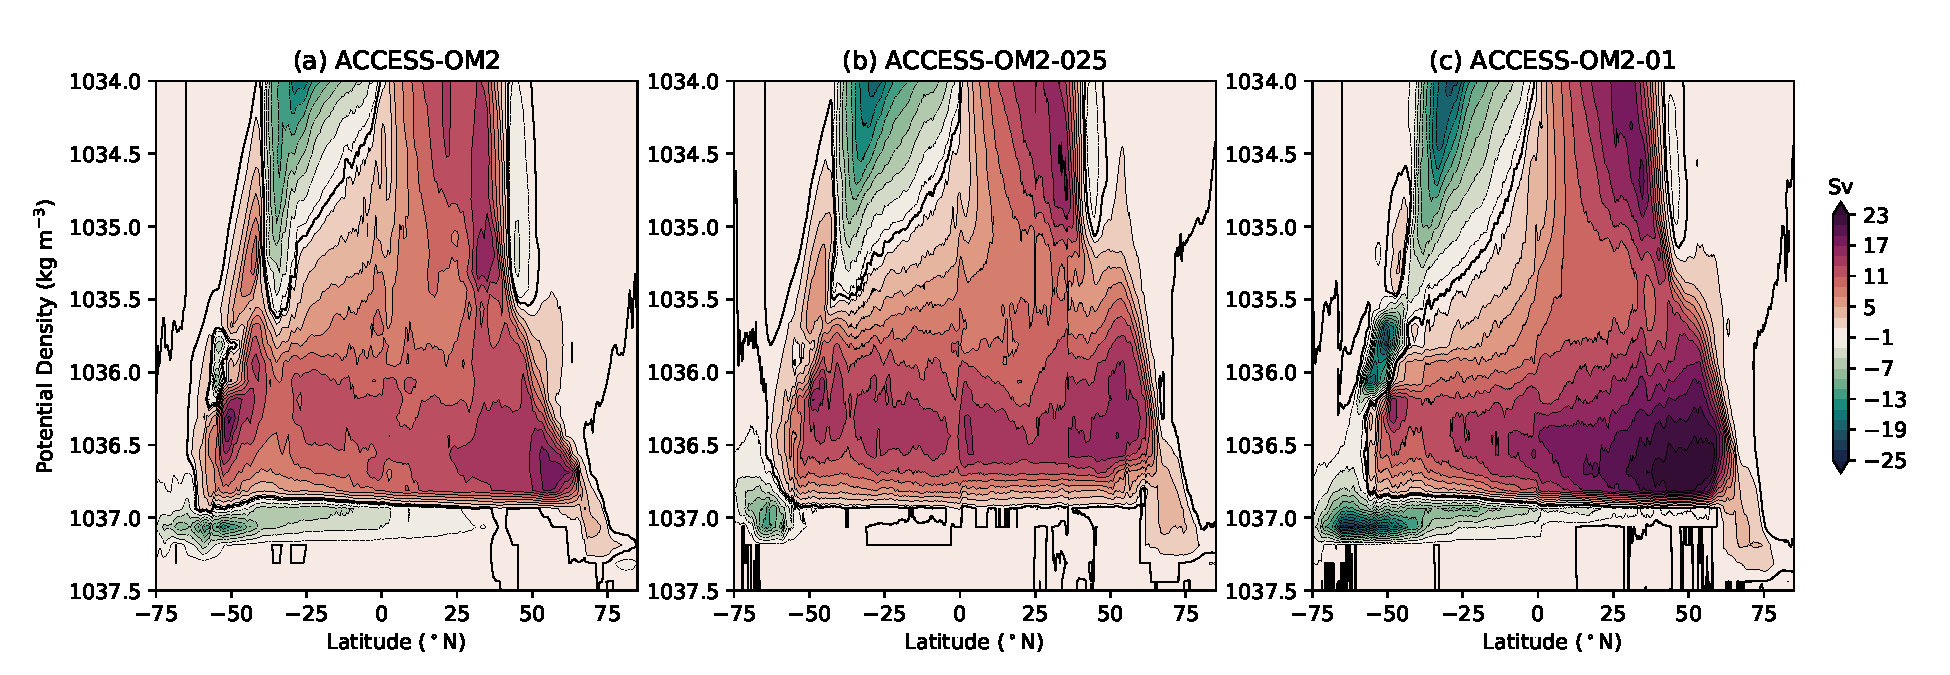
\includegraphics[width=\textwidth]{figures/overturning_circulation/mean_overturning.pdf}
\caption{Global overturning circulation on density surfaces ($\sigma_2$) for ACCESS-OM2 simulations at (a) 1$^\circ$ resolution; (b) 0.25$^\circ$ resolution and (c) 0.1$^\circ$ resolution.}
\label{F:meanoverturning}
\end{figure}


\citet{FarnetiDownesGriffiesMarslandBehrensBentsenBiBiastochBoning2015a}

\subsection{Meridional heat transport}
\CONTRIBUTORS{Ryan Holmes}

AMOC: do transect at 26.5N to cf RAPID array \url{http://www.rapid.ac.uk/rapidmoc/}
\citet{SmeedJoseyBeaulieuJohnsMoatFrajka-WilliamsRaynerMeinenBaringer2018a}

cf. \citet{NewsomBitzBryanAbernatheyGent2016a}?

\subsection{Model bias assessments}
Minimal model bias important for BOM for data assimilation in oceanMAPS, but is difficult to assess with repeat-year forcing as the mean of RYF is not climatology, so after many repeats of RYF the  slowly-adjusting ocean features will match neither climatology nor the state in the repeat year, even if the model itself is unbiased.
% -see  /Users/andy/Documents/COSIMA/COSIMA workshop 26-27 May 2016/Gary Brassington (BoM) Brassington_Ocean_modelling_and_forecasting_v3.pptx.pdf

cf BRAN

cf  \citet{KerryPowellRoughanOke2016a}

\subsection{Water mass properties and structure}
mixed layer depth - Sallee et al JGR 2013 - climate models tend to underestimate winter mld

use Argo data

and MEOP southern ocean seal data \url{http://www.meop.net}

\subsubsection{T/S diagrams}
\subsubsection{Deep water formation rates, locations, properties}
\citet{FarnetiDownesGriffiesMarslandBehrensBentsenBiBiastochBoning2015a}

\subsection{Heat conservation, bias and drift}
\CONTRIBUTORS{Chris Chapman, Ryan Holmes}

use XBT data from Chris Chapman?

cf FAFMIP? \citet{GregoryETAL2016a}

\subsubsection{SST bias}
\subsubsection{lat/depth T sections and bias}
\subsubsection{Drift: depth/time T hovmollers}
\subsubsection{zonally averaged surface heat flux terms}

\subsection{Salt conservation, bias and drift}
cf FAFMIP? \citet{GregoryETAL2016a}
\subsubsection{SSS bias}
\subsubsection{lat/depth S sections and bias}
\subsubsection{Drift: depth/time S hovmollers}
\subsubsection{zonally averaged surface salt/freshwater flux terms}

\subsection{Variability}
\citet{DanabasogluYeagerKimBehrensBentsenBiBiastochBleckBoning2016a}
%\subsubsection{ENSO}
%\subsubsection{IOD}
%\subsubsection{SAM}
\subsubsection{Western boundary current variability}
\subsubsection{EKE spatial distribution and wavenumber spectrum}
also check EKE spectrum to see if it follows the expected slope - eg \citet{CapetMcWilliamsMolemakerShchepetkin2008a}
cf. spectrum obs: \citet{XuFu2011a}

\subsection{Sea level}
\citet{GriffiesYinDurackGoddardBatesBehrensBentsenBiBiastoch2014a}

\subsection{Sea ice}

wavy ice features in 0.25deg --- poor EVP convergence? \url{https://github.com/OceansAus/access-om2/issues/87}

Too much ice south of Svalbard in 0.10deg --- \TODO{check Gulf Stream in 0.1deg --- is it carrying heat far enough north?}

\TODO{put probe points at narrowest point of northern Nares Str between Greenland and Ellesmere - compare ice export to \citet{KwokToudal-PedersenGudmandsenPang2010a}}


Reanalyses for possible comparison with model (from Helen Beggs' email 21 Mar 2018):
\begin{itemize}
\item Reanalyses of sea ice observations: The OSI-SAF reanalysis is available in ~10 km resolution from:
\url{http://osisaf.met.no/p/ice/index.html#conc-reproc}
It covers the period from 1978 to 2009 with consistent algorithm processing. 
PUM and validation reports are available at the website as well.
OSI-SAF Daily sea ice concentration analyses are being ingested into the new Decadal OFAM Climate Model by Sakov and Sandery.
\item \url{http://osisaf.met.no}: ice concentration, edge, drift and emissivity on both hemispheres, as well as climate consistent time series
\item  Bremen/Hamburg University and their AMSR2 based products
\item NCEP (Bob Grumbine), \url{http://polar.ncep.noaa.gov/seaice/} - BoM uses NCEP 1/12$^\circ$ Daily Global Sea Ice Analyses as operational inputs into their SST analyses, used as the boundary condition to the NWP models
\end{itemize}

\url{http://psc.apl.uw.edu/research/projects/arctic-sea-ice-volume-anomaly/}

thickness: \url{http://psc.apl.uw.edu/sea_ice_cdr/}

see Ice\_Validation\_ACCESS-OM2-01.ipynb \url{https://github.com/aekiss/cosima-cookbook/blob/master/notebooks/Ice_Validation_ACCESS-OM2-01.ipynb}
uses data from \url{http://nsidc.org}
%# TODO: update both to v3
%ObsDir = '/g/data/v45/akm157/data/NSIDC/NOAA_G02202_v2_conc_monthly/'  # from http://nsidc.org/data/G02202
%ObsDirExt = '/g/data/v45/akm157/data/NSIDC/NOAA_G02135_extent_monthly/'  # from http://nsidc.org/data/g02135

see SIMIP \citet{NotzJahnHollandHunkeMassonnetStroeveTremblayVancoppenolle2016a}
 
see \citet{ToyotaKimura2018a}

and check convergence \citet{BouillonFichefetLegatMadec2013a, KimmritzDanilovLosch2015a, LoschDanilov2012a, LemieuxTremblay2009a}

\citet{WangIlicakGerdesDrangeAksenovBaileyBentsenBiastochBozec2016a}

\citet{DownesFarnetiUotilaGriffiesMarslandBaileyBehrensBentsenBi2015a}

cf \citet{HeilMassomAllisonWorby2011a}
\ISSUE{3}
\subsubsection{Seasonal cycle of extent, coverage and thickness distribution}
\ISSUE{1}
\ISSUE{2}

NOAA/NSIDC Climate Data Record of Passive Microwave Sea Ice Concentration, Version 3 \url{http://nsidc.org/data/G02202}

Sea Ice Index, Version 3 \url{http://nsidc.org/data/g02135} 
See Figure~\ref{F:icevolumecategories}: the growth of Arctic ice volume is due to increasing category 5, presumably due to ridging.
We use \param{kcatbound=0}, so lower bound of ice categories is 0, 0.64, 1.39, 2.47, 4.57m \citep[][table~2]{HunkeLipscombTurnerJefferyElliott2015a-CICE5p1}.
So by year 9 most of the ice volume (not area) is more than 4.57m thick, including in the summer minimum.

\begin{figure}[ht]
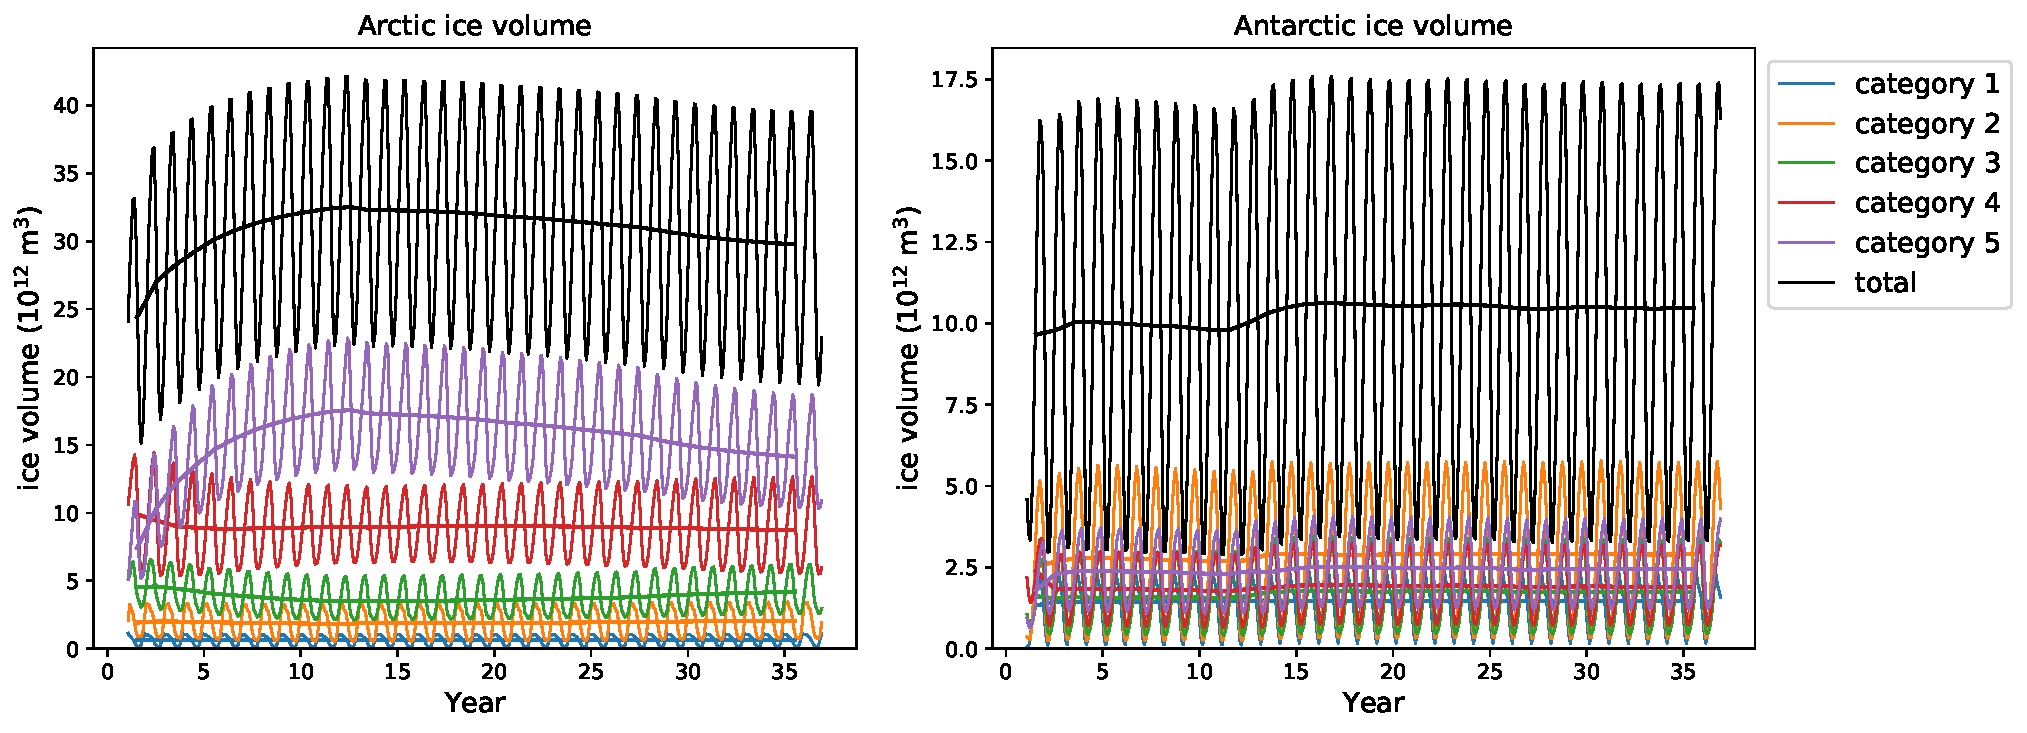
\includegraphics[width=\textwidth]{figures/ice_validation/ice_volume_categories.pdf}
\caption{Ice volume in each category at 0.1$^\circ$ resolution. The solid line shows the annual average.}
\label{F:icevolumecategories}
\end{figure}

\subsubsection{Age}
\subsubsection{Formation rate}
ice production rate in coastal polynyas \citep{TamuraOhshimaNihashi2008a,TamuraOhshima2011a,TamuraOhshimaFraserWilliams2016a,NihashiOhshima2015a,OhshimaNihashiIwamoto2016a}
- see Adele's email 9 Mar 2018 - includes a script and netcdf version.
Looks like you can download the data set here:
\url{http://www.lowtem.hokudai.ac.jp/wwwod/polar-seaflux/}
what diagnostics give us production in CICE? f_congel gives basal growth -- not relevant?
meltb, meltl,melts, meltt?
frazil?



\subsubsection{Drift}

\subsubsection{Ice deformation}
cf. \citet{HutchingsRobertsGeigerRichter-Menge2011a}

\subsubsection{Polynyas}


\citet{UotilaOFarrellMarslandBi2013a}
\citet{GirardWeissMolinesBarnierBouillon2009a}
\citet{KwokHunkeMaslowskiMenemenlisZhang2008a}


\subsection{Particularly important regions}

\subsubsection{ACC}

transport

EKE
\citet{FarnetiDownesGriffiesMarslandBehrensBentsenBiBiastochBoning2015a}

\subsubsection{North Atlantic}
North Atlantic mean state \citet{DanabasogluYeagerBaileyBehrensBentsenBiBiastochBoningBozec2014a}
and variability \citet{DanabasogluYeagerKimBehrensBentsenBiBiastochBleckBoning2016a}

\subsubsection{Arctic Ocean / Greenland-Iceland-Norway (GIN) Seas}

mixed layer depth

water properties

bottom water formation

bottom water transport over sills

\citet{WangIlicakGerdesDrangeAksenovBaileyBentsenBiastochBozec2016b}
\citet{IlicakDrangeWangGerdesAksenovBaileyBentsenBiastochBozec2016a}

\subsubsection{Pacific}
\citet{TsengLinChenThompsonBentsenBoningBozecCassouChassignet2016a}

\subsubsection{ITF}
transports through straits - cf INSTANT array obs and 
\citet{SprintallWijffelsMolcardJaya2009a, HautalaSprintallPotemraChongPandoeBrayIlahude2001a}

Marsland 12 Apr 2018: ACCESS (1$^\circ$) used Rayleigh drag to shift transport from westernmost to easternmost strait to match obs. Also cf. 
Perth-Jakarta line (XBT?)

\subsubsection{Agulhas}
transport, structure, variability
 
\appendix
\section{Auto-generated namelists}


% \newcommand{\nmldiffer}[1]{#1} % no special display of differing variables
%\newcommand{\nmldiffer}[1]{\textbf{#1}} % bold display of differing variables
\definecolor{hilite}{cmyk}{0, 0, 0.9, 0}\renewcommand{\nmldiffer}[1]{\colorbox{hilite}{#1}}\setlength{\fboxsep}{0pt} % colour highlight of differing variables (requires color package)
\renewcommand{\nmllink}[2]{#1} % don't link variables
% \newcommand{\nmllink}[2]{\href{https://github.com/mom-ocean/MOM5/search?q=#2}{#1}} % link variables to documentation (requires hyperref package)
%\newcommand{\nml}[1]{{\small\textsf{\input{local/#1}}}} % use nml tables generated from local files
\renewcommand{\nml}[1]{{\small\textsf{\input{raijin/#1}}}} % use nml tables generated on raijin
%\newlength{\nmllen}\setlength{\nmllen}{13ex}

These are auto-generated by make\_nml\_tables.py which uses nmltab (\url{https://github.com/aekiss/nmltab}).
Variables are weblinks to source code searches. 
Variables that differ between the models are \nmldiffer{\textcolor{link}{highlighted}}.
\ignored{Greyed values} are ignored. % (greying only works in groups with use_this_module shown, so typically doesn't work for tables of differences).

\FIXME{these namelists are out of date}

\TODO{generate complete tables that include the default values of parameters not specified in namelists}

\rowcolors{1}{lightblue}{white}

\subsection{MOM namelist `input.nml'}\label{S:mom-namelist}
\renewcommand{\nmllink}[2]{\href{https://github.com/mom-ocean/MOM5/search?q=#2}{#1}} % link to documentation (requires hyperref package)
\nml{input_nml.tex}

\subsection{CICE namelists}\label{S:cice-namelist}
\renewcommand{\nmllink}[2]{\href{https://github.com/OceansAus/cice5/search?q=#2}{#1}} % link to documentation (requires hyperref package)
\subsubsection{cice\_in.nml}
\nml{cice_in_nml.tex}
\subsubsection{input\_ice.nml}
\nml{input_ice_nml.tex}
\subsubsection{input\_ice\_gfdl.nml}
\nml{input_ice_gfdl_nml.tex}
\subsubsection{input\_ice\_monin.nml}
\nml{input_ice_monin_nml.tex}

\subsection{MATM namelist `input\_atm.nml'}\label{S:matm-namelist}
\renewcommand{\nmllink}[2]{\href{https://github.com/OceansAus/matm/search?q=#2}{#1}} % link to documentation (requires hyperref package)
\nml{input_atm_nml.tex}

\section{Auto-generated tables of namelist changes within runs}
%\renewcommand{\nmldiffer}[1]{#1} % no special display of differing variables
%\runchanges{access-om2-01/01deg_jra55v13_ryf8485_spinup1}
%\runchanges{access-om2-01/01deg_jra55v13_ryf8485_spinup2}
%\runchanges{access-om2-01/01deg_jra55v13_ryf8485_spinup3}
%\runchanges{access-om2-01/01deg_jra55v13_ryf9091_spinup1}
%\runchanges{access-om2-025/025deg_jra55_ryf_broadwell_test}
%\runchanges{access-om2-025/025deg_jra55_ryf_spinup1}
%\runchanges{access-om2-025/025deg_jra55_ryf_spinup2}
%\runchanges{access-om2-025/025deg_jra55_ryf_spinup3}
%\runchanges{access-om2-025/025deg_jra55_ryf_spinup4}
%\runchanges{access-om2-025/025deg_jra55_ryf_spinup5}
%\runchanges{access-om2-025/025deg_jra55_ryf_spinup6}
%\runchanges{access-om2-025/025deg_jra55_ryf_spinup7}
%\runchanges{access-om2-025/025deg_jra55_ryf_spinup7_RCP45}
%\runchanges{access-om2-025/025deg_jra55v13_ryf8485_gmredi}
%\runchanges{access-om2-025/025deg_jra55v13_ryf8485_redi}
%\runchanges{access-om2-025/025deg_jra55v13_ryf8485_redi2}
%\runchanges{access-om2-025/025deg_jra55v13_ryf8485_redi3}
%\runchanges{access-om2-025/025deg_jra55v13_ryf8485_spinup_A}
%\runchanges{access-om2/1deg_core_nyf_spinup_A}
%\runchanges{access-om2/1deg_jra55_ryf8485_spinup1}
%\runchanges{access-om2/1deg_jra55_ryf8485_spinup2}
%\runchanges{access-om2/1deg_jra55_ryf_RCP45}
%\runchanges{access-om2/1deg_jra55_ryf_spinup1}
%\runchanges{access-om2/1deg_jra55_ryf_spinup2}
%\runchanges{access-om2/1deg_jra55_ryf_spinup3}
%\runchanges{access-om2/1deg_jra55_ryf_spinup4}
%\runchanges{access-om2/1deg_jra55_ryf_spinup5}
%\runchanges{access-om2/1deg_jra55_ryf_spinup6}
%\runchanges{access-om2/1deg_jra55_ryf_spinup7}
%\runchanges{access-om2/1deg_jra55_ryf_spinup8}
%\runchanges{access-om2/1deg_jra55_ryf_spinup9}
%\runchanges{access-om2/1deg_jra55v13_ryf0304_RCP45}
%\runchanges{access-om2/1deg_jra55v13_ryf0304_spinup_A}
%\runchanges{access-om2/1deg_jra55v13_ryf8485_RCP45}
%\runchanges{access-om2/1deg_jra55v13_ryf8485_spinup_A}
%\runchanges{access-om2/1deg_jra55v13_ryf9091_RCP45}
%\runchanges{access-om2/1deg_jra55v13_ryf9091_spinup_A}

\section{Auto-generated tables of namelist differences from ACCESS, ACCESS-CM2, ACCESS-ESM, OFAM}\label{S:namelist-model-comparisons}

\subsection{ACCESS-OM2-01 MOM compared to OFAM3}

\subsection{ACCESS-OM2-01 MOM compared to MOM-SIS-01 and GFDL}

\subsection{ACCESS-OM2-01 CICE compared to RASM and NCAR}\label{S:rasm-namelist}
ice_in_RASM  \TODO{get permisssion}
ncar_ice_in  \TODO{get permisssion}

\bibliographystyle{ametsoc2014}
\bibliography{ACCESS-OM2-1-025-010deg}

\end{document}  
